\chapter{Interesting Directions}
\label{chap:future}


% % \subsubsection{Sampling}
% % The input for the neural network is a discrete representation. In this sense,} sampling is a way to create a representation of a function based on its values at certain points of the domain. From the point of view of Representation Theory, we can interpret this as a projection of the function onto the primal Shannon basis (i.e., Dirac delta distribution). In the context of signal processing, this basis is a sampling grid of impulses and the representation consists of the sequence of signal values at the grid locations.

% % One important aspect of sampling for learning signals with coordinate-based neural network is the structure of the sampling grid. In that respect, it is instrumental to consider two types of grid structures: Regular and Irregular. See Fig~\ref{f:sampling}. {\color{red}The sampling mode is stored in the MR-Structure, so it can be taken into account when doing operations that modify the sampling grid.}

% % \begin{figure}[!h]
% % \centering
% % 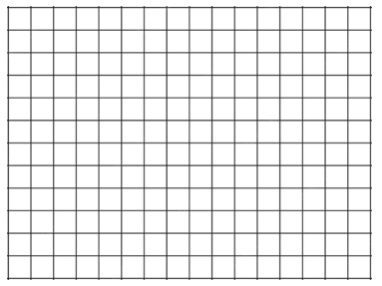
\includegraphics[width=0.42\linewidth]{img/ch4/regular.png}
% % \hfil
% % 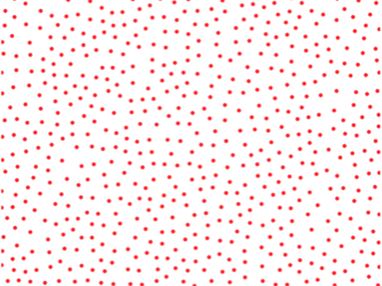
\includegraphics[width=0.42\linewidth]{img/ch4/poisson.png}
% % \\
% % {\hfil (regular grid) \hfil\hfil (irregular grid) \hfil}
% % \caption{Sampling Modes}
% % \label{f:sampling}
% % \end{figure}


% % \subsubsection{Filtering}

% % The input of signal values to the network can be filtered to separate it into different frequency bands. In this sense, we can use the unfiltered signal, a low-pass version of the signal or a band-pass version of the signal. See Fig~\ref{f:filter}.

% % It is common to employ a Gaussian Kernel as the low-pass Kernel and a Difference of Gaussians as the band-pass kernel.

% % \begin{figure}[!h]
% % \centering
% % 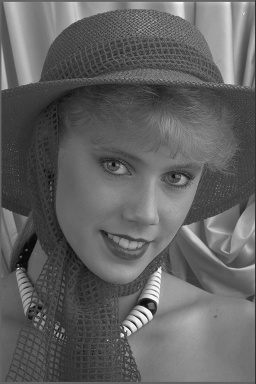
\includegraphics[width=0.30\linewidth]{img/ch4/signal.png}
% % 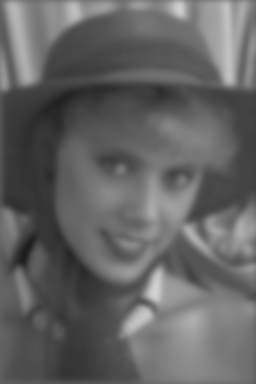
\includegraphics[width=0.30\linewidth]{img/ch4/gaussian.png}
% % 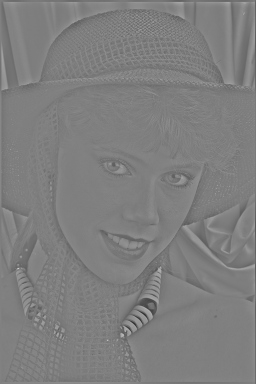
\includegraphics[width=0.30\linewidth]{img/ch4/laplacian.png}\\
% % {\hfil \hfil signal \hfil \hfil \hfil low-pass \hfil \hfil \hfil band-pass \hfil}
% % \caption{Filter Types}
% % \label{f:filter}
% % \end{figure}

% % \subsubsection{multi-stage stack}

% % A Multiresolution Stack consists of a hierarchy of sampling grids with different resolutions. The standard grid structure form a dyadic lattice of regular grids obeying the $2^j$ rule, i.e., each level of the grid has twice the size of the previous one. 
% % Nonetheless, it is also possible to define a irregular multiresolution grid structure. In this case, each resolution level has approximately twice the number of random sample points of the previous level (see Fig~\ref{f:multi}(b)).
% % On the other hand, it is possible to have a stack of sampling grid with the same resolution, in which the signal is the same at each level or is filtered (see Fig~\ref{f:multi}(a)). Section~\ref{s:lod} gives more details on this option.
% % \begin{figure}[!h]
% % \centering
% % 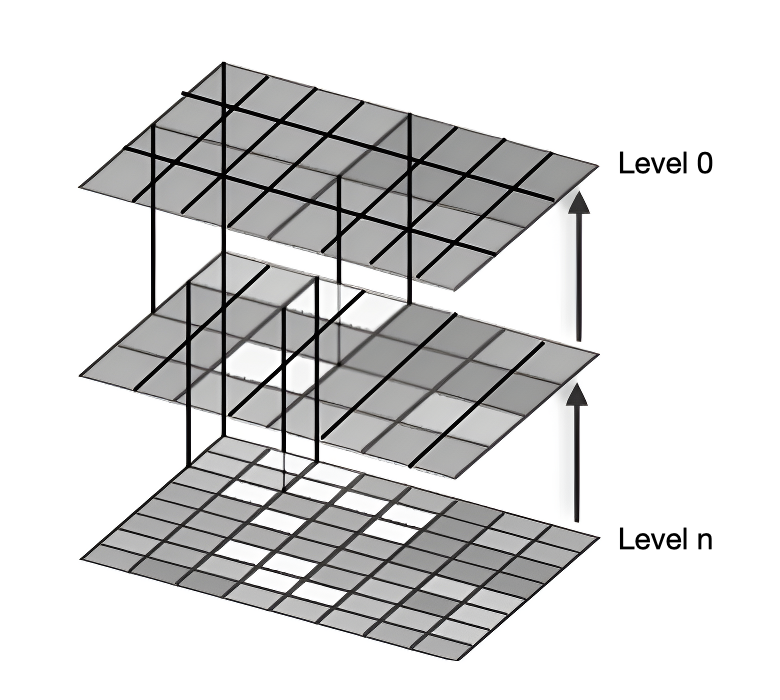
\includegraphics[width=0.45\linewidth]{img/ch4/tower.png}
% % 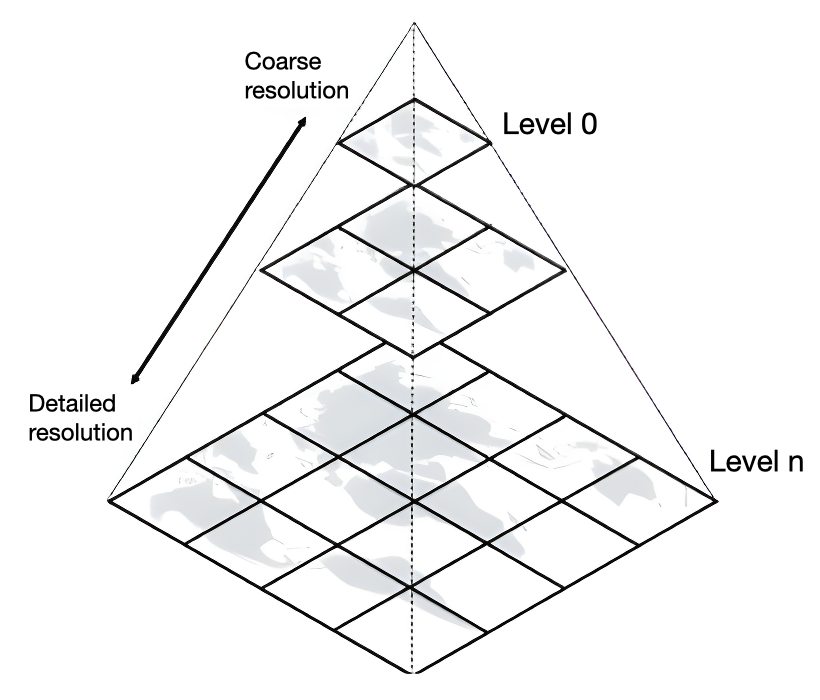
\includegraphics[width=0.45\linewidth]{img/ch4/pyramid.png}\\
% % {\hfil tower \hfil \hfil \hfil pyramid \hfil}
% % \vspace{-0.2cm}
% % \caption{\hl{Multiresolution Hierarchies}}
% % \label{f:multi}
% % \end{figure}


% % \subsection{Solid Texture Mapping}

% % Solid textures offer practical advantages as they eliminate the need for computing $uv$-coordinates on a surface. We trained a solid texture of a marble using Perlin Noise as described in section \ref{s-multires-3d}, and we integrated our representation into the Omniverse platform, which provides a comprehensive rendering pipeline management system. Figure \ref{f:solid_texture_mapping} showcases some of the results achieved using our solid texture mapping approach.

% % \begin{figure}[!h]
% % \centering
% % 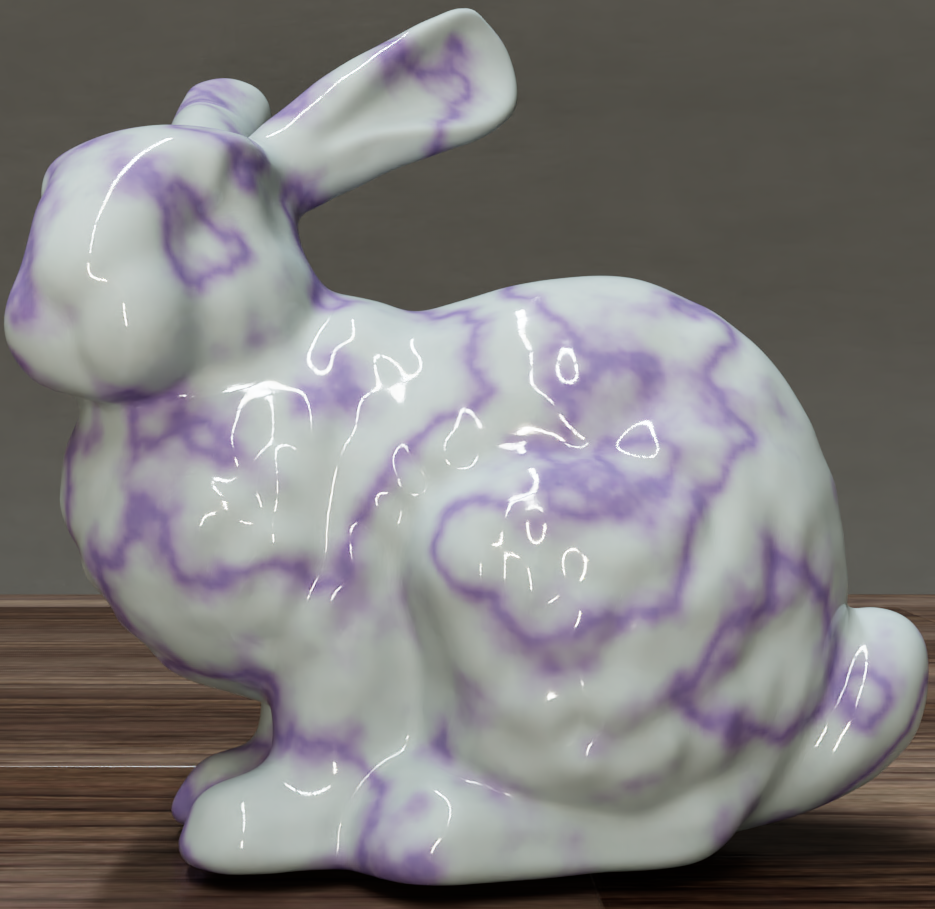
\includegraphics[width=0.375\linewidth]{img/omniverse/bunny_mrnet.0000.png}
% % 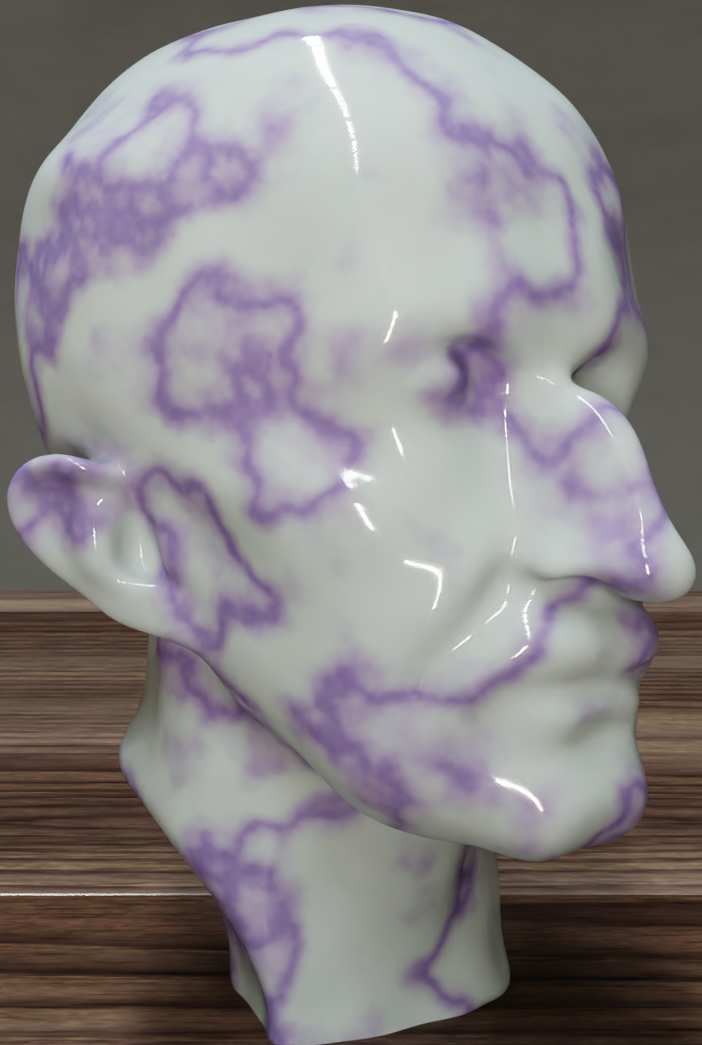
\includegraphics[width=0.245\linewidth]{img/omniverse/max_plank_mrnet_512_mc400.0099.png}
% % 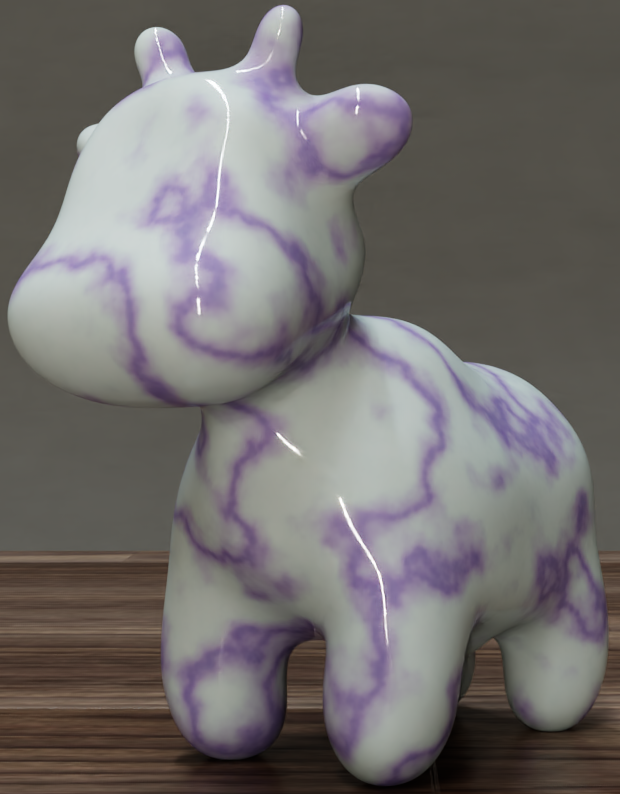
\includegraphics[width=0.285\linewidth]{img/omniverse/spot_mrnet.0101.png}
% % \caption{Solid Texture Mapping.}
% % \label{f:solid_texture_mapping}
% % \end{figure}

% % To apply the solid texture, we extract meshes from implicit surfaces represented by neural networks and perform the inference of the texture network at the vertices of the mesh. We render the scene using \textit{path tracing}, and we can choose among various materials and shading options to enhance the visual quality of the scene. This demonstrates that this approach can be fully integrated in the  graphics pipeline.

% % \end{comment}